\subsection{Kubernetes as a Docker containers orchestration system}
\textit{This subchapter describes what Kubernetes is and what problems it solves. Furthermore, the chapter acknowledges Kubernetes popularity and briefly introduces chosen Kubernetes objects.}
~\\
~\\
The process of deploying multiple containers of one application can be optimized through automation. This kind of automation is referred to as \textbf{orchestration} \cite{art-byza}.

There was a need to automatically deploy and manage a large number of services at global scale on millions of servers. Thus, Google developed Borg. Borg is a private orchestration system. It is very powerful, but also very much coupled to Google’s own internal and proprietary technologies. Therefore, in 2014 Google launched a new project called: \textbf{Kubernetes}. The name comes from a Greek word which means "helmsman, pilot". Apart from Kubernetes, there are alternative solutions invented, other orchestrators, but Kubernetes \textbf{won the orchestration wars} \cite{book-cndwk,article-modelling-performance-k8s}.

"Kubernetes does the things that the very best system administrator would do: automation, failover, centralized logging, monitoring. It takes what we’ve learned in the DevOps community and makes it the default, out of the box." These are the words uttered by Kelsey Hightower --- a Google employee with legendary contributions to Kubernetes \cite{book-cndwk}.

Kubernetes was built \textbf{to make deployments easy, to reduce the time and effort} which needs to be poured into them. To achieve this goals, Kubernetes offers \textbf{a wide variety of features}\cite{k8s,book-cndwk,article-state-machine}:
\begin{itemize}
\item creating, destroying, replicating containers,
\item rolling updates of containers,
\item built-in health checks (liveness and readiness probes),
\item autoscaling,
\item redundancy and failover --- to make the applications deployed on top of Kubernetes more resilient and reliable,
\item being provider-agnostic --- Kubernetes can be deployed on-premises and in the cloud and in both cases it will provide the same set of features, thus, it may be said that Kubernetes unifies the underlying infrastructure,
\item utilizing provider-specific (sometimes referred to as: vendor-specific) features, e.g. AWS load balancer or Google Cloud load balancer,
\item self-healing,
\item service discovery,
\item load balancing,
\item storage orchestration.
\end{itemize}


Kubernetes is the first project of the CNCF \cite{article-state-machine}. Kubernetes is already \textbf{used by some well-known entities}, e.g. NASA \cite{nasa}, F-16 jets \cite{online-f16}, Zalando \cite{online-zalando}, ING \cite{online-ing}, booking.com \cite{online-bookingcom}. Apart from that, the \textbf{Kubernetes popularity is growing}, basing on the information from CNCF Survey 2019, which states that 78\% of respondents use Kubernetes in production and that this is a huge jump from 58\% using in the previous --- 2018 year \cite{cncf-2019}. Even the older CNCF Survey from year 2017 shows Kubernetes as number one cloud management platform --- it it presented in figure \ref{fig:cncf-con}.

\begin{figure}[H]
    \centering
    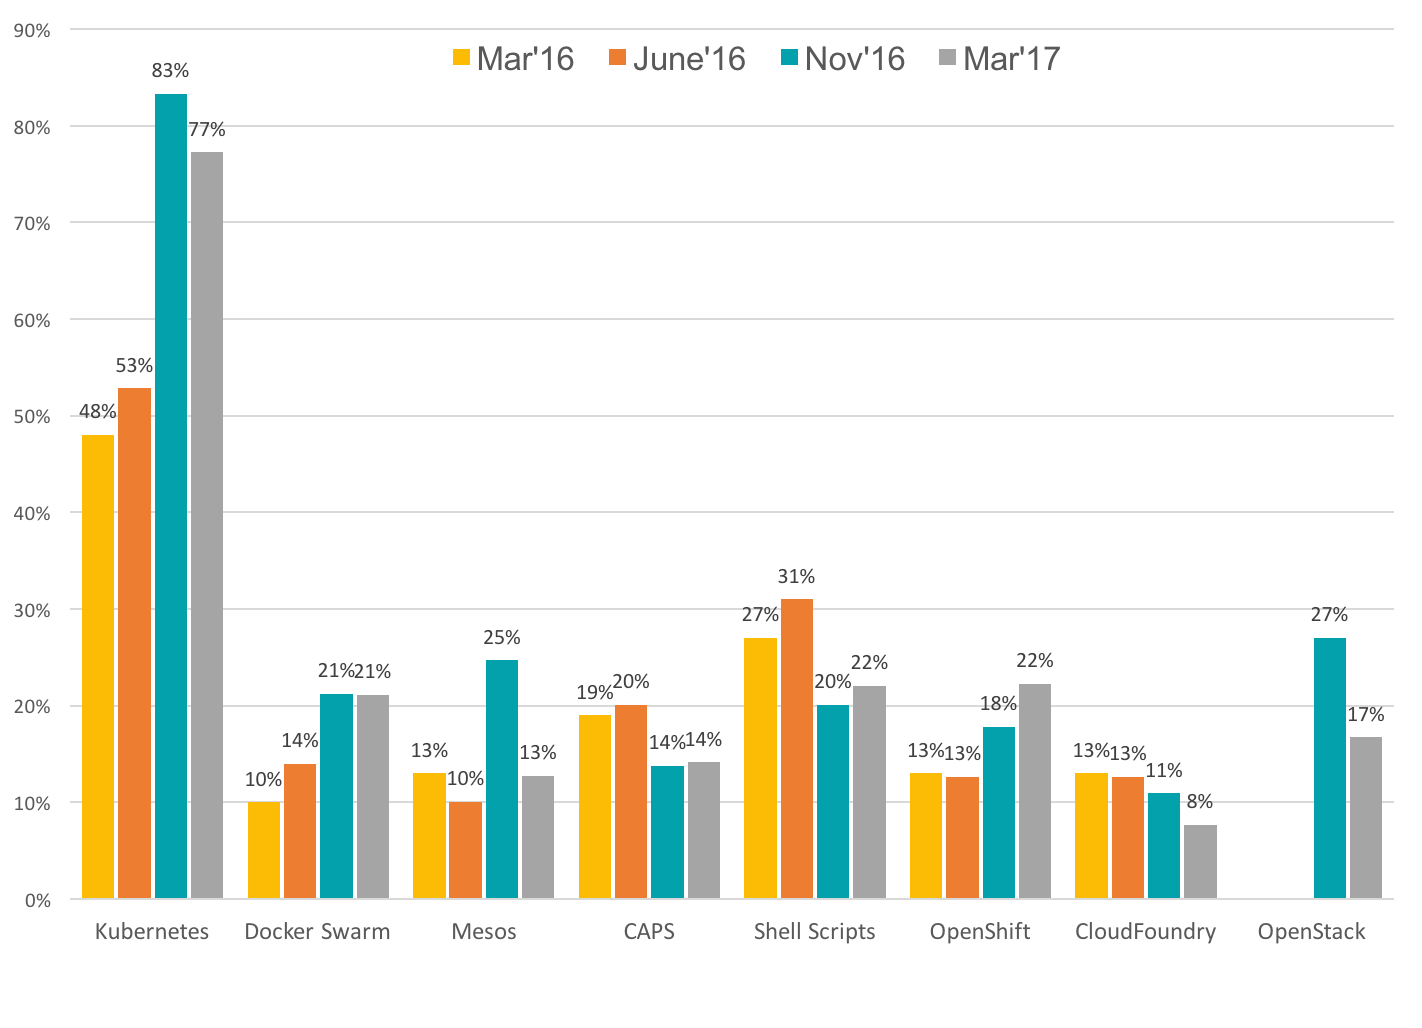
\includegraphics[width=12cm]{figures/cncf-container-orchestrators.png}
    \captionsetup{justification=centering,margin=2cm}
    \caption{Results of CNCF Survey from year 2017 showing Kubernetes as number one cloud management platform \cite{cncf-2017}}
    \label{fig:cncf-con}
\end{figure}

The \textbf{basic working unit in Kubernetes is a pod}. A pod is an abstraction and it represents one application, a set of containers. Two things are crucial to know about pods \cite{article-modelling-performance-k8s}:
\begin{itemize}
\item all the containers defined in a pod will be deployed on one machine,
\item a pod has one IP address assigned and all the containers defined in this pod share the same IP address.
\end{itemize}

A pod is all that is needed to deploy a set of containers. Pod is a Kubernetes object and there are many more objects, for example: deployment, replica sets, service, ingress. The important thing to note is that these \textbf{objects can be configured in a declarative way}, thanks to YAML files \cite{k8s-declarative}.

Kubernetes provides mechanisms for maintaining, deploying, healing and scaling containerized microservices. Thanks to that, Kubernetes hides the complexity of microservices orchestration. It is much easier to satisfy non-functional requirements of microservices deployment by using Kubernetes. An example of such requirements may be: availability, healing, redundancy or autoscaling \cite{article-k8s-as-avail}.

\subsection{Kubernetes architecture}
% this short summary before each subchapter helps me to stay focused on what i want to write about
\textit{This subchapter contains a high level description of the Kubernetes architecture. The focus is on the responsibilities of each Kubernetes component.}

\subsubsection{Kubernetes cluster}
A \textbf{Kubernetes cluster} may be defined as a collection of storage and networking resources which are used by Kubernetes to run various workloads \cite{book-mastering-k8s}. Another definition states that a Kubernetes cluster is a single unit of computers which are connected to work together and which are provisioned with Kubernetes components \cite{k8s-cluster}.

A cluster consists of two kinds of instances: masters and nodes. An instance can be a virtual machine or a physical computer \cite{article-k8s-as-avail,k8s-cluster}. This is depicted in figure ~\ref{fig:cluster-k8s}. Kubernetes nodes communicate with Kubernetes master.
\begin{figure}[H]
    \centering
    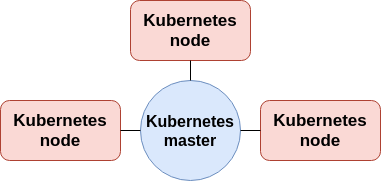
\includegraphics[width=10cm]{figures/cluster-k8s.png}
    \caption{Kubernetes cluster diagram depicting a master-slave architecture}
    \label{fig:cluster-k8s}
\end{figure}

\subsubsection{Masters and nodes}
\textbf{The role of the master is to manage the cluster}. This means that master: schedules applications, maintains their desired state, scales them, handles events, manages nodes. \textbf{Nodes serve as the worker machines}. They are responsible for running containers and handling container operations. Masters schedule containers to run on nodes \cite{book-mastering-k8s, k8s-cluster}. At least one node and one master is needed in a Kubernetes cluster. In order to provide fault-tolerance and high availability in production environments, multiple master and multiple node instances are run \cite{k8s-components}.

The instances in a Kubernetes cluster (masters and nodes) are hosts to several \textbf{Kubernetes components}. There are \textbf{master components}, used to control the cluster and there are also \textbf{node components}, run on each node. All the components are presented in figure \ref{fig:components-of-kubernetes}:
\begin{figure}[H]
    \centering
    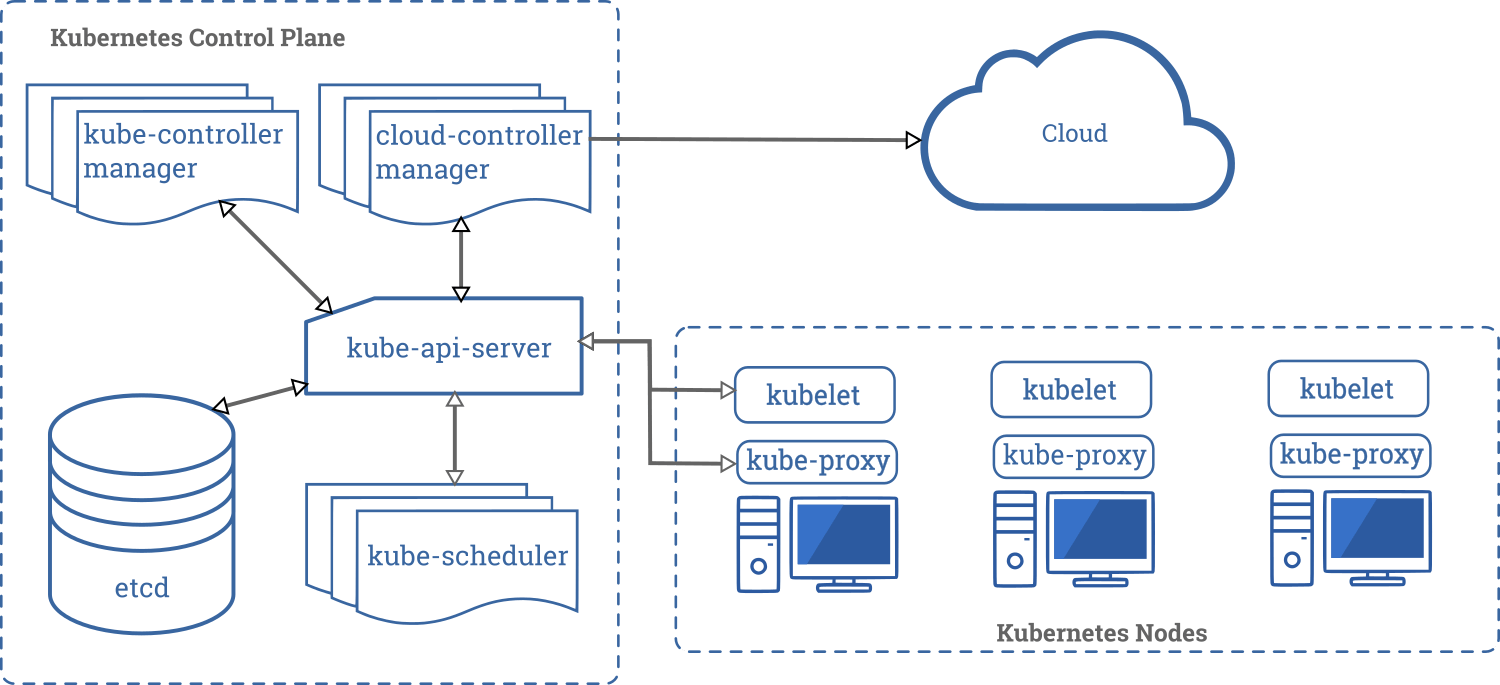
\includegraphics[width=14cm]{figures/components-of-kubernetes.png}
    \caption{Kubernetes components including master and node components \cite{k8s-components}}
    \label{fig:components-of-kubernetes}
\end{figure}


\subsubsection{Components}
The master components are also known as the control plane’s components. They are as follows \cite{book-mastering-k8s, k8s-components}:
\begin{itemize}
\item Etcd (a key-value store),
\item API server,
\item Scheduler,
\item Controller manager and Cloud Controller manager.
\end{itemize}

\paragraph{}
\textbf{Etcd} stores the entire cluster state. It is a highly-available key-value store. It is enough, for a test Kubernetes cluster, to deploy one instance of Etcd. However, for the purposes of high availability and redundancy, a 3-node or even 5-node Etcd cluster is typical. It is recommended to have a back up plan for the data stored in Etcd\cite{book-mastering-k8s,k8s-components}. The name \textit{etcd} follows a naming convention within the UNIX directory structure. In UNIX, all system configuration files are contained in a folder called "/etc". The last letter "d" stands for "distributed" \cite{etcd-name}.

\textbf{API server} exposes the Kubernetes REST API. It allows the nodes to communicate with the master and it also allows end users to interact with the cluster. Thanks to the fact that API server is stateless and that all its data is stored in etcd, API server can easily scale horizontally. The main implementation of a Kubernetes API server is kube-apiserver\cite{book-mastering-k8s,k8s-components,k8s-cluster}.


\textbf{Scheduler} is responsible for assiging containers to nodes. Scheduler selects a node for a container to run on. It considers a range of factors: resource requirements, various constraints, affinity and anti-affinity specifications, data locality, inter-workload interference, and deadlines. The implementation is known as kube-scheduler \cite{book-mastering-k8s, k8s-components}.

\textbf{Controller manager} runs controller processes such as: watching the shared state of the cluster and making changes needed to move the current state into the desired state. Controller manager is a collection of separate managers, but they are all compiled into a single binary and run in a single process in order to reduce complexity. The controllers consist of: Node Controller, Replication Controller, Endpoints Controller, Service Account and Token Controllers. The implementation of Controller manager is kube-controller-manager \cite{book-mastering-k8s, k8s-components}.

\textbf{Cloud Controller manager} interacts with a specified underlying cloud provider (e.g. Amazon Web Services or Google Cloud Platform). It is implemented by cloud-controller-manager and therefore, it allows the Kubernetes code and the cloud vendor’s code to evolve independently \cite{k8s-components}.

As aforementioned, there are also node components. They run on both: masters and nodes. They are as follows \cite{book-mastering-k8s, k8s-components}:
\begin{itemize}
\item Kubelet,
\item Proxy,
\item Container Runtime.
\end{itemize}

\textbf{Kubelet} oversees the communication with the master components (by monitoring API server for changes) and makes sure that containers, described by a Pod, are running and healthy (so it manages a Pod lifecycle). A Pod is a simple object from a Kubernetes API and it represents a set of containers. Containers which were not created by Kubenernetes are not managed by Kubelet \cite{book-mastering-k8s, k8s-components}.

\textbf{Proxy} is implemented by kube-proxy. It is a network proxy and it implements a part of the Kubernetes Service concept, which means that it is responsible for exposing an application as a network service and it provides load balancing \cite{book-mastering-k8s, k8s-components}.

\textbf{Container Runtime} is the software which is responsible for operating containers. Several container runtimes are supported: Docker, containerd, CRI-O, and any implementation of the Kubernetes CRI (Container Runtime Interface). It is a design policy of Kubernetes that is ought to be decoupled from a specific container runtime. Under some circumstates it should be possible to switch from one container runtime to another or to use multiple of them at once. Originally, Kubernetes was designed to manage only Docker containers \cite{book-mastering-k8s, k8s-components}.

\subsubsection{Other services}
\label{k8s-other-services}
Apart from master and node components, there are also \textbf{add-ons, extensions, and third party tools} which communicate with Kubernetes by the API server and which provide additional functionality. Examples of such services are: DNS, Vertical Pod Autoscaler, Cluster Autoscaler, Istio, Kubernetes Dashboard, kube-ops-view, node-problem-detector, etc \cite{book-cndwk}}.

\subsubsection{The Kubernetes networking model}
\label{k8s-net}
Kubernetes states a few \textbf{networking requirements} \cite{k8s-net}:
\begin{itemize}
\item pods on a node must be able to communicate with all pods on all nodes without Network Address Translation (NAT),
\item agents on a node (e.g. system daemons, kubelet) must be able to communicate with all pods on that node.
\end{itemize}

There are many available options that help with satisfying these requirements, e.g. AWS VPC CNI for Kubernetes, Azure CNI for Kubernetes, Flannel, OpenVSwitch, Project Calico, etc \cite{k8s-net}. CNI stands for Container Networking Interface and it is a specification and also a set of libraries for writing network plugins to configure network interfaces in Linux containers. A CNI container is bound to have its own IP address. For Kubernetes, \textbf{each pod has its own IP address}, so the pod is the CNI container \cite{book-mastering-k8s}. \textbf{Containers that belong to a one pod share the same IP address}, which means that these containers can reach all reach each other’s ports on localhost and also that none two containers should expose the same port. This model is known as "IP-per-pod" \cite{k8s-net}.
